\chapter{感情ベクトルの出力例}

本手法で得られる感情ベクトルの出力例を以下に示す.
\begin{figure}[H]
	\begin{tabular}{cc}
		\begin{minipage}[t]{0.45\hsize}
			\centering
			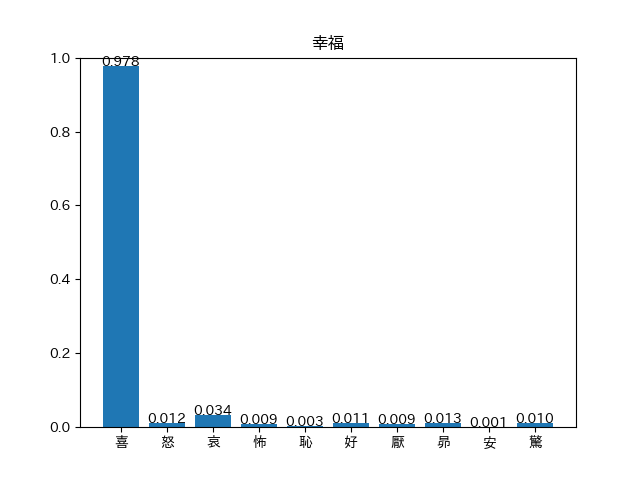
\includegraphics[keepaspectratio, scale=0.45]{./figure/BERT+weight/Q05/001.png}
			\subcaption{「幸福」に対する感情ベクトル}
		\end{minipage} &
		\begin{minipage}[t]{0.45\hsize}
			\centering
			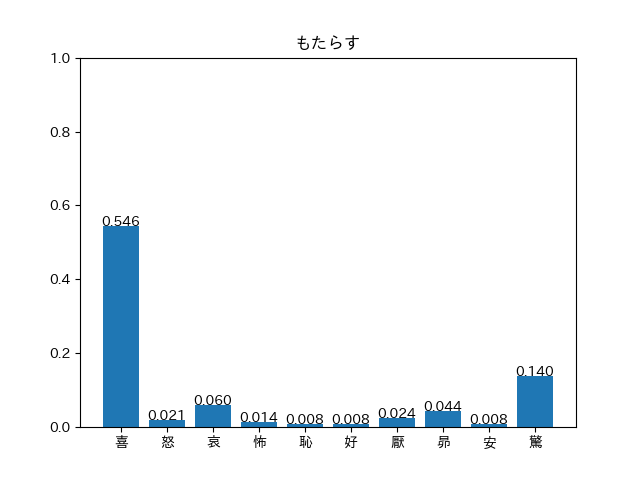
\includegraphics[keepaspectratio, scale=0.45]{./figure/BERT+weight/Q05/002.png}
			\subcaption{「もたらす」に対する感情ベクトル}
		\end{minipage} \\
		\begin{minipage}[t]{0.45\hsize}
			\centering
			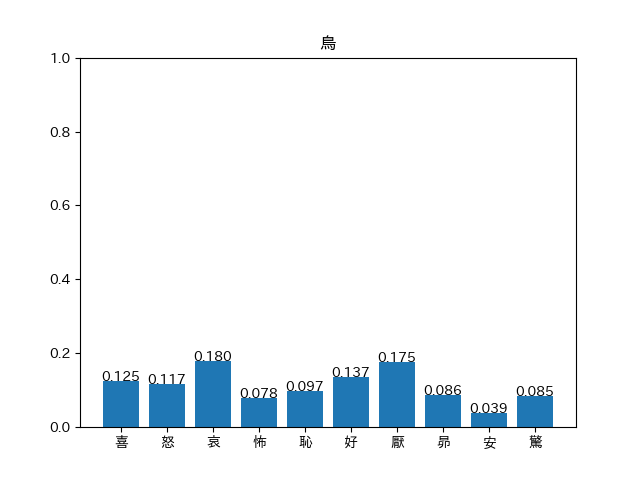
\includegraphics[keepaspectratio, scale=0.45]{./figure/BERT+weight/Q05/003.png}
			\subcaption{「鳥」に対する感情ベクトル}
		\end{minipage} \\
	\end{tabular}
	\caption{「幸福をもたらす鳥.」に対する各単語の感情ベクトル}
	\label{fig:output_q05}
\end{figure}

\begin{figure}[H]
	\begin{tabular}{cc}
		\begin{minipage}[t]{0.45\hsize}
			\centering
			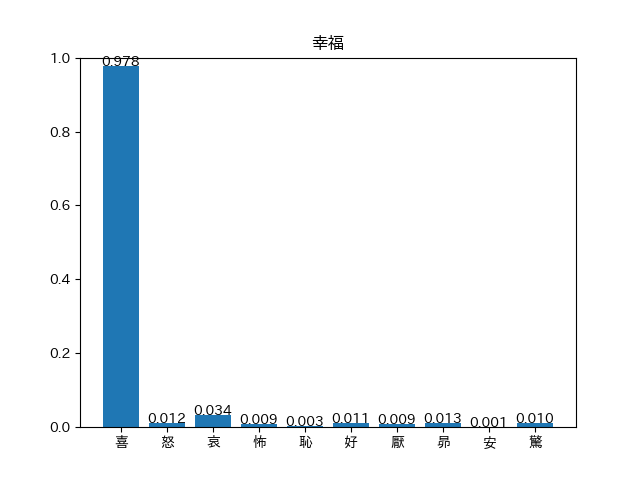
\includegraphics[keepaspectratio, scale=0.45]{./figure/BERT+weight/Q05/001.png}
			\subcaption{「不運」に対する感情ベクトル}
		\end{minipage} &
		\begin{minipage}[t]{0.45\hsize}
			\centering
			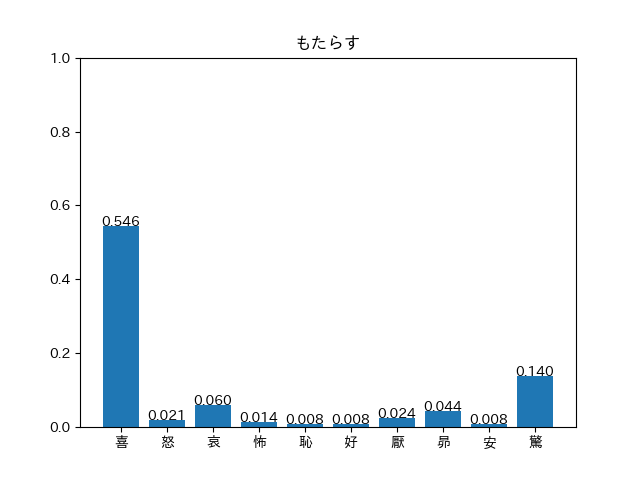
\includegraphics[keepaspectratio, scale=0.45]{./figure/BERT+weight/Q05/002.png}
			\subcaption{「もたらす」に対する感情ベクトル}
		\end{minipage} \\
		\begin{minipage}[t]{0.45\hsize}
			\centering
			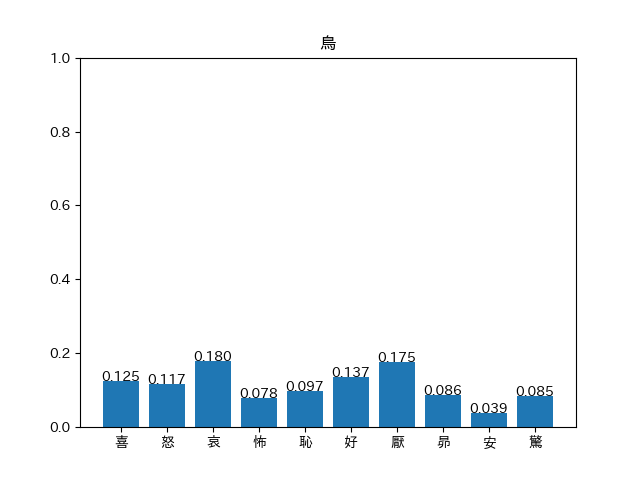
\includegraphics[keepaspectratio, scale=0.45]{./figure/BERT+weight/Q05/003.png}
			\subcaption{「行い」に対する感情ベクトル}
		\end{minipage} \\
	\end{tabular}
	\caption{「不運をもたらす行い.」に対する各単語の感情ベクトル}
	\label{fig:output_q06}
\end{figure}

\begin{figure}[H]
	\begin{tabular}{cc}
		\begin{minipage}[t]{0.45\hsize}
			\centering
			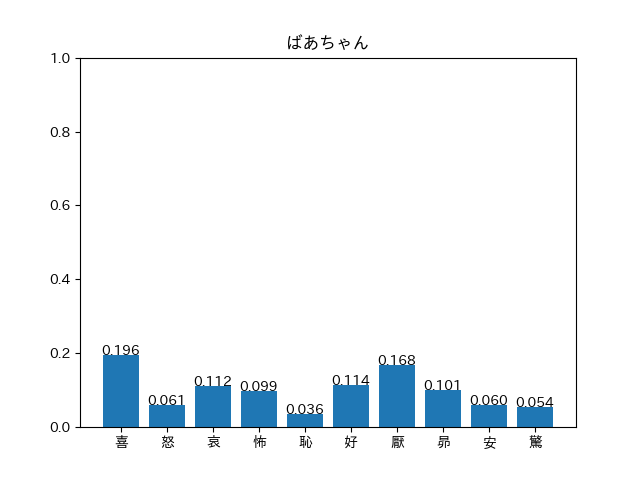
\includegraphics[keepaspectratio, scale=0.45]{./figure/BERT+weight/Q11/001.png}
			\subcaption{「ばあちゃん」に対する感情ベクトル}
		\end{minipage} &
		\begin{minipage}[t]{0.45\hsize}
			\centering
			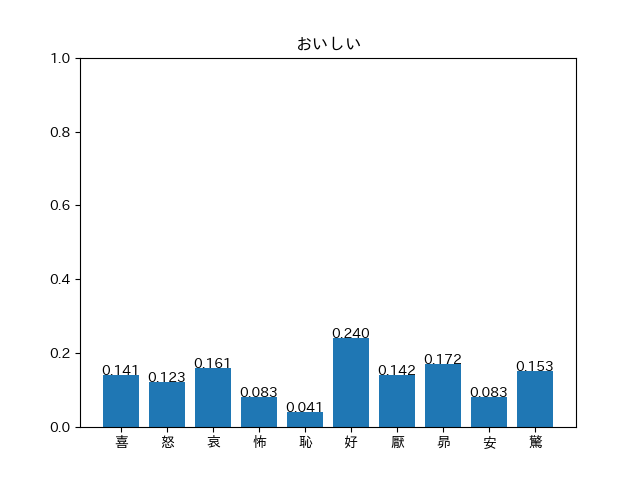
\includegraphics[keepaspectratio, scale=0.45]{./figure/BERT+weight/Q11/002.png}
			\subcaption{「おいしい」に対する感情ベクトル}
		\end{minipage} \\
		\begin{minipage}[t]{0.45\hsize}
			\centering
			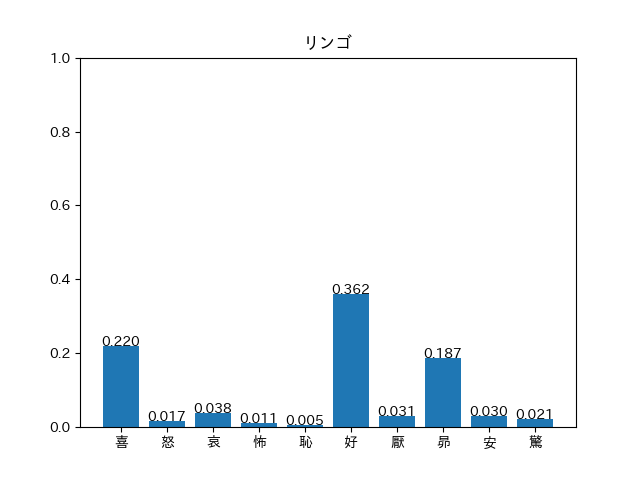
\includegraphics[keepaspectratio, scale=0.45]{./figure/BERT+weight/Q11/003.png}
			\subcaption{「リンゴ」に対する感情ベクトル}
		\end{minipage} &
		\begin{minipage}[t]{0.45\hsize}
			\centering
			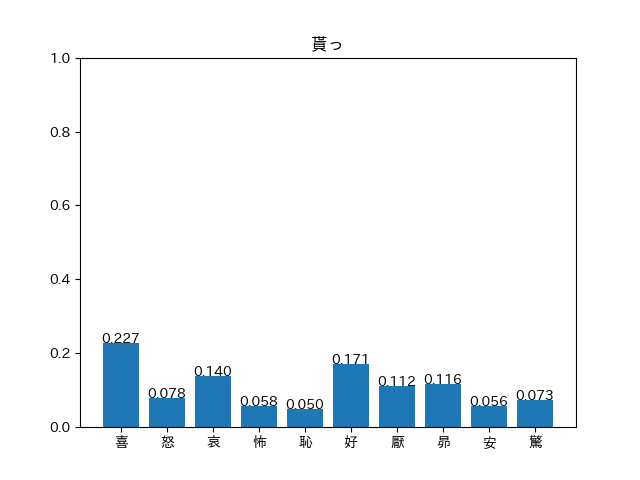
\includegraphics[keepaspectratio, scale=0.45]{./figure/BERT+weight/Q11/004.png}
			\subcaption{「貰っ」に対する感情ベクトル}
		\end{minipage} \\
	\end{tabular}
	\caption{「おばあちゃんからおいしいリンゴを貰った.」に対する各単語の感情ベクトル}
	\label{fig:output_q11}
\end{figure}

\begin{figure}[H]
	\begin{tabular}{cc}
		\begin{minipage}[t]{0.45\hsize}
			\centering
			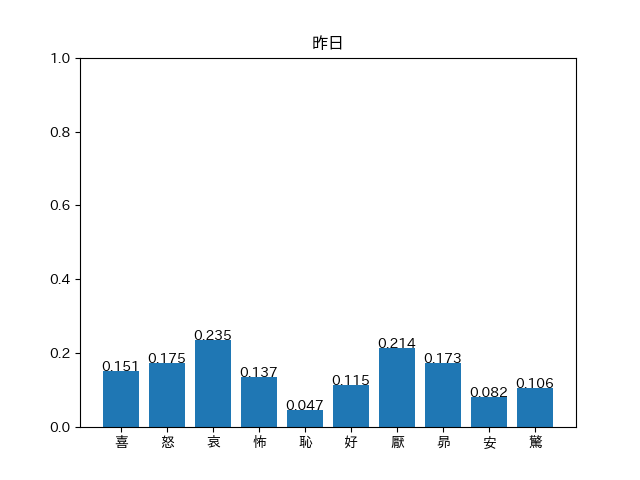
\includegraphics[keepaspectratio, scale=0.45]{./figure/BERT+weight/Q12/001.png}
			\subcaption{「昨日」に対する感情ベクトル}
		\end{minipage} &
		\begin{minipage}[t]{0.45\hsize}
			\centering
			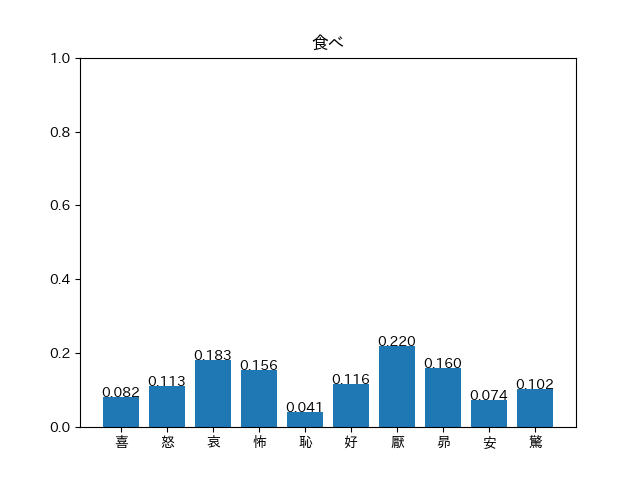
\includegraphics[keepaspectratio, scale=0.45]{./figure/BERT+weight/Q12/002.png}
			\subcaption{「食べ」に対する感情ベクトル}
		\end{minipage} \\
		\begin{minipage}[t]{0.45\hsize}
			\centering
			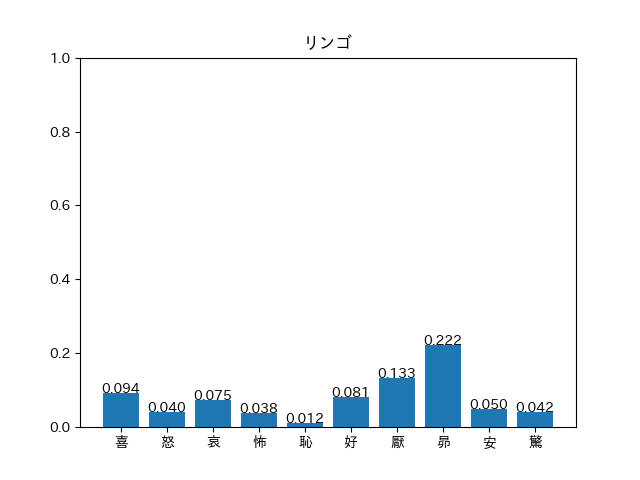
\includegraphics[keepaspectratio, scale=0.45]{./figure/BERT+weight/Q12/003.png}
			\subcaption{「リンゴ」に対する感情ベクトル}
		\end{minipage} &
		\begin{minipage}[t]{0.45\hsize}
			\centering
			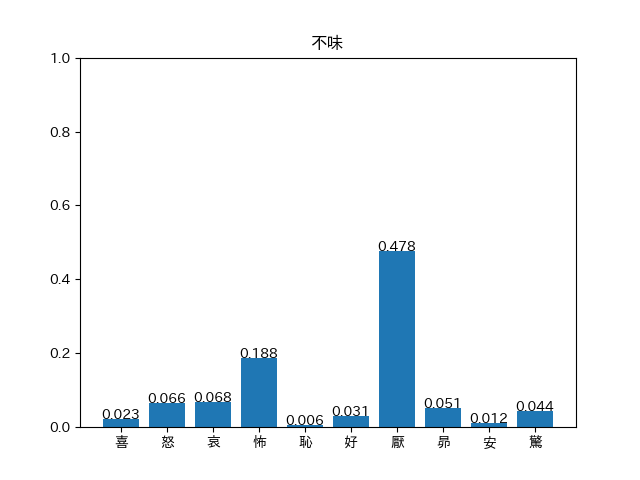
\includegraphics[keepaspectratio, scale=0.45]{./figure/BERT+weight/Q12/004.png}
			\subcaption{「不味」に対する感情ベクトル}
		\end{minipage} \\
	\end{tabular}
	\caption{「昨日食べたリンゴが不味すぎた.」に対する各単語の感情ベクトル}
	\label{fig:output_q12}
\end{figure}
